\documentclass{beamer}
\usepackage{ctex}
\usepackage{tikz,tikz-3dplot}
\usetheme{focus}
\tikzset{
    global scale/.style={scale=#1,every node/.append style={scale=#1}},
    CC1/.style ={circle,minimum width = 30pt, minimum height =30pt, draw},
    CC2/.style ={circle,minimum width = 30pt, minimum height =30pt, draw, fill=blue!20},
    RA1/.style ={rectangle,minimum width = 30pt, minimum height =20pt, draw},
    RA2/.style ={rectangle,minimum width = 1cm, minimum height = 1cm, draw},
    SU/.style ={very near start,sloped,above}}

\begin{document}
\begin{frame}{1-1}
    \begin{tikzpicture}[every node/.style={rectangle,minimum width = 3.5cm,draw}]
        \node(1)  at (0,2) {数学/离散数学};
        \node(2)  at (0,-2) {大学生程序设计竞赛};
        \node(3)  at (-4,1) {C语言程序设计};
        \node(4)  at (-4,0) {算法分析与设计I};
        \node(5)  at (-4,-1) {数据结构};
        \node(6)  at (4,1) {数据分析与可视化};
        \node(7)  at (4,0) {最优化理论};
        \node(8)  at (4,-1) {数据挖掘};
        \node(9) [fill=blue!20,minimum height = 1.5cm] at (0,0) {算法分析与设计II}
            edge [<-,thick,dashed](1) 
            edge [->,thick,dashed](2) 
            edge [<-,thick](3) 
            edge [<-,thick](4) 
            edge [<-,thick](5) 
            edge [->,thick](6) 
            edge [->,thick](7) 
            edge [->,thick](8);
    \end{tikzpicture}
\end{frame}
\begin{frame}{2-1}
    \tdplotsetmaincoords{70}{110}
    \begin{tikzpicture}[scale=2,tdplot_main_coords]
        \foreach \i in {0,1,2,3,4}
        \foreach \j in {0,1}{
            \draw[fill=white,fill opacity=0.5] (0+\j,0+\i,0) -- (0+\j,1+\i,0) -- (0+\j,1+\i,1) -- (0+\j,0+\i,1) -- cycle;
            \draw[fill=white,fill opacity=0.5] (0+\j,0+\i,0) -- (1+\j,0+\i,0) -- (1+\j,1+\i,0) -- (0+\j,1+\i,0) -- cycle;
            \draw[fill=white,fill opacity=0.5] (0+\j,0+\i,0) -- (1+\j,0+\i,0) -- (1+\j,0+\i,1) -- (0+\j,0+\i,1) -- cycle;
            \draw[fill=white,fill opacity=0.5] (1+\j,0+\i,0) -- (1+\j,1+\i,0) -- (1+\j,1+\i,1) -- (1+\j,0+\i,1) -- cycle;
            \draw[fill=white,fill opacity=0.5] (0+\j,1+\i,0) -- (1+\j,1+\i,0) -- (1+\j,1+\i,1) -- (0+\j,1+\i,1) -- cycle;
            \draw[fill=white,fill opacity=0.5] (1+\j,0+\i,1) -- (1+\j,1+\i,1) -- (0+\j,1+\i,1) -- (0+\j,0+\i,1) -- cycle;}
    \end{tikzpicture}
\end{frame}
\begin{frame}{2-2}
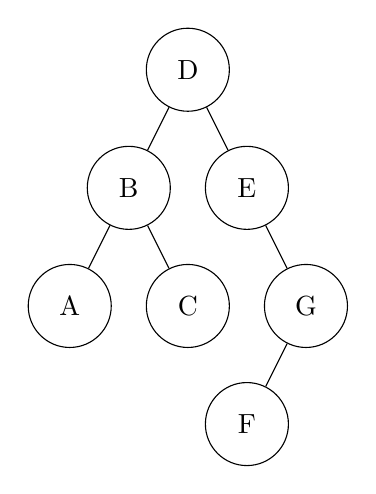
\begin{tikzpicture}[every node/.style={circle,minimum width = 30pt, minimum height =30pt, draw}]
    \node{D}
        child{node{B}
            child{node{A}}
            child{node{C}}}
        child{node{E}
            child[missing]{}
            child{node{G}
                child{node{F}
                child[missing]{}}
                child[missing]{}}};
\end{tikzpicture}
\end{frame}
\begin{frame}{2-4}
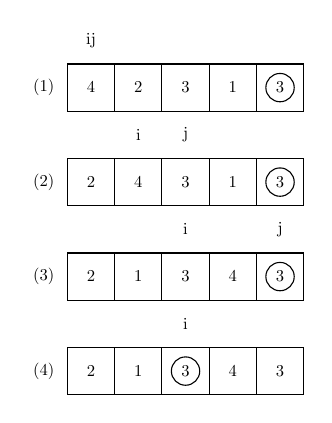
\begin{tikzpicture}[global scale=.6]
    \draw (-1,0) node{(4)};
    \draw (0,0) node[RA2]{2};
    \draw (1,0) node[RA2]{1};
    \draw (2,0) circle(.3) node[RA2]{3};
    \draw (3,0) node[RA2]{4};
    \draw (4,0) node[RA2]{3};
    \draw (2,1) node{i};
    \draw (-1,2) node{(3)};
    \draw (0,2) node[RA2]{2};
    \draw (1,2) node[RA2]{1};
    \draw (2,2) node[RA2]{3};
    \draw (3,2) node[RA2]{4};
    \draw (4,2) circle(.3) node[RA2]{3};
    \draw (2,3) node{i};
    \draw (4,3) node{j};
    \draw (-1,4) node{(2)};
    \draw (0,4) node[RA2]{2};
    \draw (1,4) node[RA2]{4};
    \draw (2,4) node[RA2]{3};
    \draw (3,4) node[RA2]{1};
    \draw (4,4) circle(.3) node[RA2]{3};
    \draw (1,5) node{i};
    \draw (2,5) node{j};
    \draw (-1,6) node{(1)};
    \draw (0,6) node[RA2]{4};
    \draw (1,6) node[RA2]{2};
    \draw (2,6) node[RA2]{3};
    \draw (3,6) node[RA2]{1};
    \draw (4,6) circle(.3) node[RA2]{3};
    \draw (0,7) node{ij};
\end{tikzpicture}
\end{frame}
\begin{frame}{2-5}
    \begin{tikzpicture}[
        hv/.style={to path={-| (\tikztotarget)},->,thick},
        h/.style={dashed,thick}]
        \draw (1,1) node[RA2]{1};
        \node[RA2](1) at(2,1) {3};
        \node[RA2](2) at(3,1) {4};
        \node[RA2](3) at(4,1) {6};
        \node[RA2](4) at(5,1) {7};
        \draw (6,1) node[RA2]{8};
        \draw (7,1) node[RA2]{10};
        \draw (8,1) node[RA2]{13};
        \draw (9,1) node[RA2]{14};
        \node (5) at (4,2.5) {4<6} edge[hv] (2) edge[h] (3);
        \node (6) at (2,3.5) {4>3} edge[hv] (5) edge[h] (1);
        \node (7) at (5,4.5) {4<7} edge[hv] (6) edge[h] (4);
        \node at (5,5.5) {} edge[hv] (7);
    \end{tikzpicture}
\end{frame}
\begin{frame}{2-6}
    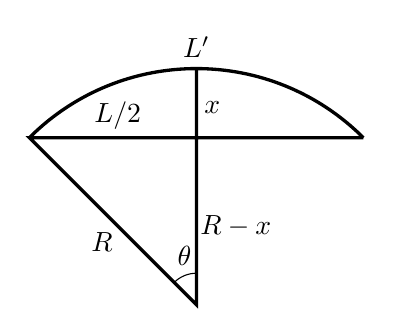
\begin{tikzpicture}
        \draw[very thick] (2.12,2.12) arc (45:135:3) node[midway,above]{$L'$};
        \draw[very thick] (0,3)--(0,0)--(-2.12,2.12)--(2.12,2.12);
        \draw (0,.4) arc (90:135:.4) node[midway,above]{$\theta$};
        \node at (.5,1){$R-x$};
        \node at (.2,2.5){$x$};
        \node at (-1,2.4){$L/2$};
        \node at (-1.2,.8){$R$};
    \end{tikzpicture}
\end{frame}
\begin{frame}{2-7}
    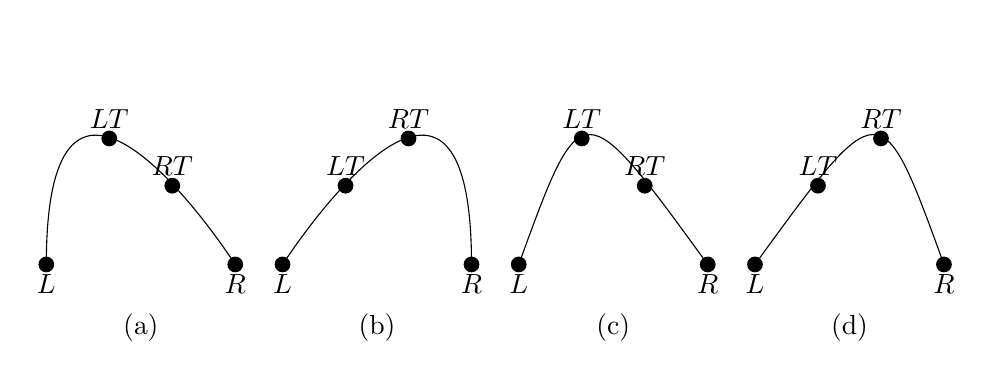
\begin{tikzpicture}
        \foreach \x in {0,1,2,3}{  
            \fill   ($(0,0)!\x*.25!(12,0)$) circle (.1) node[below]{$L$}
                    ($(2.4,0)!\x*.25!(14.4,0)$) circle (.1) node[below]{$R$}
                    ($(0.8,0)!\x*.25!(12.8,0)!abs(cos(\x*90))*.3+.5!(0.8+3*\x,2)$) circle (.1) node[above]{$LT$}
                    ($(1.6,0)!\x*.25!(13.6,0)!abs(sin(\x*90))*.3+.5!(1.6+3*\x,2)$) circle (.1) node[above]{$RT$};}
        \draw (0,0) ..controls (0,3) and (1.6,1.2)..(2.4,0);
        \draw (5.4,0) ..controls (5.4,3) and (3.8,1.2)..(3,0);
        \draw (6,0) ..controls (6.8,2.2)..(8.4,0);
        \draw (11.4,0) ..controls (10.6,2.2)..(9,0);
        \node at(1.2,-.8) {(a)};
        \node at(4.2,-.8) {(b)};
        \node at(7.2,-.8) {(c)};
        \node at(10.2,-.8) {(d)};
    \end{tikzpicture}
\end{frame}
\begin{frame}{3-1}
    \begin{tikzpicture}
        \draw (0,0) rectangle (3,0.8);
        \draw (0,1) rectangle (3,1.8);
        \draw (0,2) rectangle (3,2.8);
        \draw (-3,3.6) rectangle (0,4.4);
        \draw (3,3.6) rectangle (6,4.4);
        \draw[very thick,->] (2,3) arc (180:90:1);
        \draw[very thick,->] (0,4) arc (90:0:1);
        \node at(2.5,3.3){Pop};
        \node at(0.4,3.3){Push};
        \node at(1.5,2.4){top};
    \end{tikzpicture}
\end{frame}
\begin{frame}{3-2}
    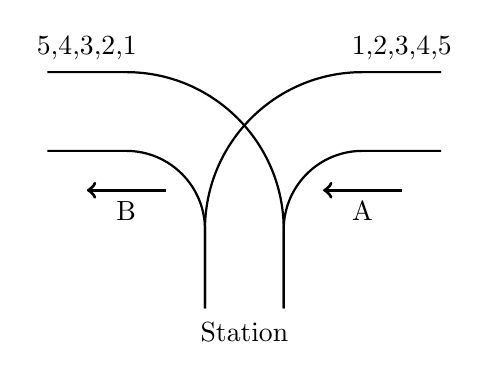
\begin{tikzpicture}
        \draw[thick] (0,0) -- (1,0) arc (90:0:2)-- (3,-3);
        \draw[thick] (0,-1) -- (1,-1) arc (90:0:1)-- (2,-3);
        \draw[thick] (5,0) -- (4,0) arc (90:180:2)-- (2,-3);
        \draw[thick] (5,-1) -- (4,-1) arc (90:180:1)-- (3,-3);
        \node at(.5,.3){5,4,3,2,1};
        \node at(4.5,.3){1,2,3,4,5};
        \node at(2.5,-3.3){Station};
        \draw[very thick,->] (1.5,-1.5) -- (0.5,-1.5) node[midway,below]{B};
        \draw[very thick,->] (4.5,-1.5) -- (3.5,-1.5) node[midway,below]{A};
    \end{tikzpicture}
\end{frame}
\begin{frame}{3-3}
    \begin{tikzpicture}
        \foreach \i in {0,...,5}{
        \draw (0+\i,0) rectangle (0.8+\i,2);}
        \draw (-1.6,1.7) rectangle (-0.8,3.7);
        \draw (6.6,0.3) rectangle (7.4,-1.7);
        \draw[very thick,->] (-1.2,1.5) arc (180:270:1);
        \draw[very thick,->] (6,1.5) arc (90:0:1);
        \node at(-1.5,.4){Enqueue};
        \node at(7,1.7){Dequeue};
        \node at(0.4,2.4){rear};
        \node at(5.4,2.4){front};
    \end{tikzpicture}
\end{frame}
\begin{frame}{4-1}
    \begin{tikzpicture}[global scale=0.65]
        \node[CC1] (1) at(0,0){$A$};
        \node[CC1] (2) at(2,2){$B_1$};
        \node[CC1] (3) at(2,0){$B_2$};
        \node[CC1] (4) at(2,-2){$B_3$};
        \node[CC1] (5) at(5,2){$C_1$};
        \node[CC1] (6) at(5,0){$C_2$};
        \node[CC1] (7) at(5,-2){$C_3$};
        \node[CC1] (8) at(8,1){$D_1$};
        \node[CC1] (9) at(8,-1){$D_2$};
        \node[CC1] (10) at(10,0){$E$};
        \draw (1) --(2) node[SU]{2};
        \draw (1) --(3) node[SU]{5};
        \draw (1) --(4) node[SU]{1};
        \draw (2) --(5) node[SU]{12};
        \draw (2) --(6) node[SU]{14};
        \draw (2) --(7) node[SU]{10};
        \draw (3) --(5) node[SU]{6};
        \draw (3) --(6) node[SU]{10};
        \draw (3) --(7) node[SU]{4};
        \draw (4) --(5) node[SU]{13};
        \draw (4) --(6) node[SU]{12};
        \draw (4) --(7) node[SU]{11};
        \draw (5) --(8) node[SU]{3};
        \draw (5) --(9) node[SU]{9};
        \draw (6) --(8) node[SU]{6};
        \draw (6) --(9) node[SU]{5};
        \draw (7) --(8) node[SU]{8};
        \draw (7) --(9) node[SU]{10};
        \draw (8) --(10) node[SU]{5};
        \draw (9) --(10) node[SU]{2};
        \node[RA1] (a) at(0,-3.5) {状态1};
        \node[RA1] (b) at(2,-3.5) {状态2};
        \node[RA1] (c) at(5,-3.5) {状态3};
        \node[RA1] (d) at(8,-3.5) {状态4};
        \node[RA1] (e) at(10,-3.5) {状态5};
        \draw[->] (a)--(b) node[midway,above]{$k_1$};
        \draw[->] (b)--(c) node[midway,above]{$k_2$};
        \draw[->] (c)--(d) node[midway,above]{$k_3$};
        \draw[->] (d)--(e) node[midway,above]{$k_4$};
    \end{tikzpicture}
\end{frame}
\begin{frame}{4-2-1}
    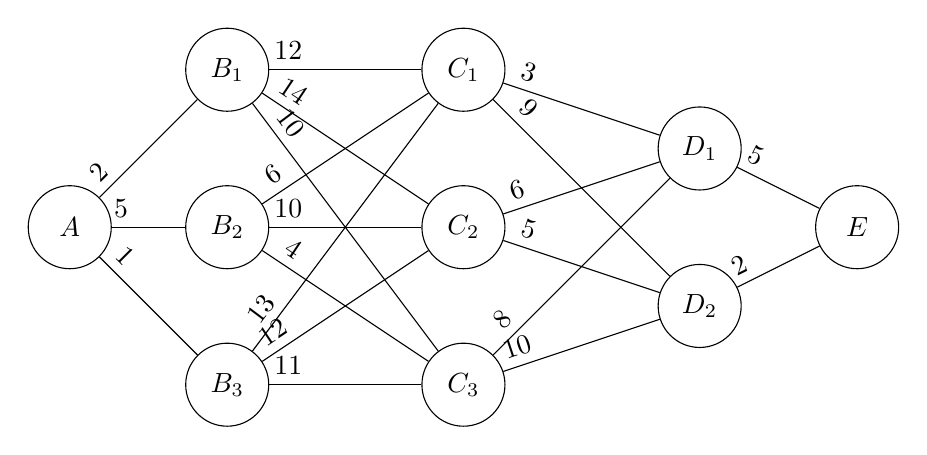
\begin{tikzpicture}
        \node[CC1] (1) at(0,0){$A$};
        \node[CC1] (2) at(2,2){$B_1$};
        \node[CC1] (3) at(2,0){$B_2$};
        \node[CC1] (4) at(2,-2){$B_3$};
        \node[CC1] (5) at(5,2){$C_1$};
        \node[CC1] (6) at(5,0){$C_2$};
        \node[CC1] (7) at(5,-2){$C_3$};
        \node[CC1] (8) at(8,1){$D_1$};
        \node[CC1] (9) at(8,-1){$D_2$};
        \node[CC1] (10) at(10,0){$E$};
        \draw (1) --(2) node[SU]{2};
        \draw (1) --(3) node[SU]{5};
        \draw (1) --(4) node[SU]{1};
        \draw (2) --(5) node[SU]{12};
        \draw (2) --(6) node[SU]{14};
        \draw (2) --(7) node[SU]{10};
        \draw (3) --(5) node[SU]{6};
        \draw (3) --(6) node[SU]{10};
        \draw (3) --(7) node[SU]{4};
        \draw (4) --(5) node[SU]{13};
        \draw (4) --(6) node[SU]{12};
        \draw (4) --(7) node[SU]{11};
        \draw (5) --(8) node[SU]{3};
        \draw (5) --(9) node[SU]{9};
        \draw (6) --(8) node[SU]{6};
        \draw (6) --(9) node[SU]{5};
        \draw (7) --(8) node[SU]{8};
        \draw (7) --(9) node[SU]{10};
        \draw (8) --(10) node[SU]{5};
        \draw (9) --(10) node[SU]{2};
    \end{tikzpicture}
\end{frame}
\begin{frame}{4-2-2}
    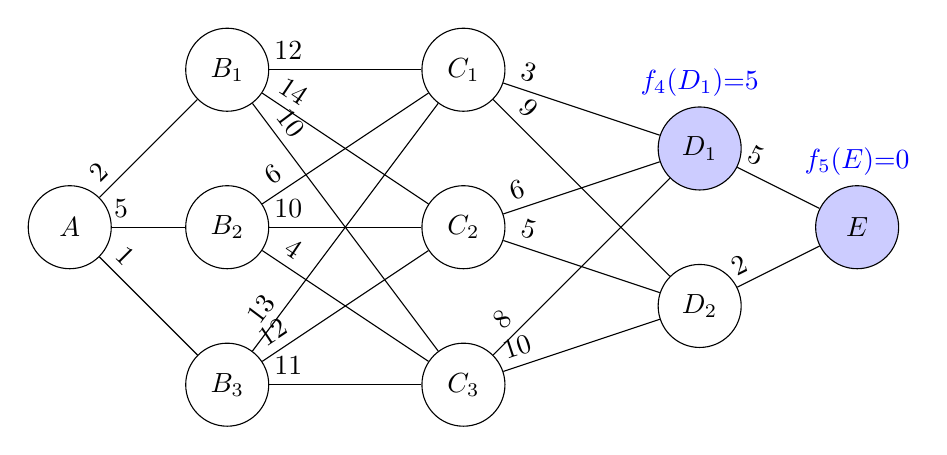
\begin{tikzpicture}[every label/.style={blue}]
        \node[CC1] (1) at(0,0){$A$};
        \node[CC1] (2) at(2,2){$B_1$};
        \node[CC1] (3) at(2,0){$B_2$};
        \node[CC1] (4) at(2,-2){$B_3$};
        \node[CC1] (5) at(5,2){$C_1$};
        \node[CC1] (6) at(5,0){$C_2$};
        \node[CC1] (7) at(5,-2){$C_3$};
        \node[CC2] (8)[label=above:$f_4(D_1){=}5$] at(8,1){$D_1$};
        \node[CC1] (9) at(8,-1){$D_2$};
        \node[CC2] (10)[label=above:$f_5(E){=}0$] at(10,0){$E$};
        \draw (1) --(2) node[SU]{2};
        \draw (1) --(3) node[SU]{5};
        \draw (1) --(4) node[SU]{1};
        \draw (2) --(5) node[SU]{12};
        \draw (2) --(6) node[SU]{14};
        \draw (2) --(7) node[SU]{10};
        \draw (3) --(5) node[SU]{6};
        \draw (3) --(6) node[SU]{10};
        \draw (3) --(7) node[SU]{4};
        \draw (4) --(5) node[SU]{13};
        \draw (4) --(6) node[SU]{12};
        \draw (4) --(7) node[SU]{11};
        \draw (5) --(8) node[SU]{3};
        \draw (5) --(9) node[SU]{9};
        \draw (6) --(8) node[SU]{6};
        \draw (6) --(9) node[SU]{5};
        \draw (7) --(8) node[SU]{8};
        \draw (7) --(9) node[SU]{10};
        \draw (8) --(10) node[SU]{5};
        \draw (9) --(10) node[SU]{2};
    \end{tikzpicture}
\end{frame}
\begin{frame}{4-2-3}
    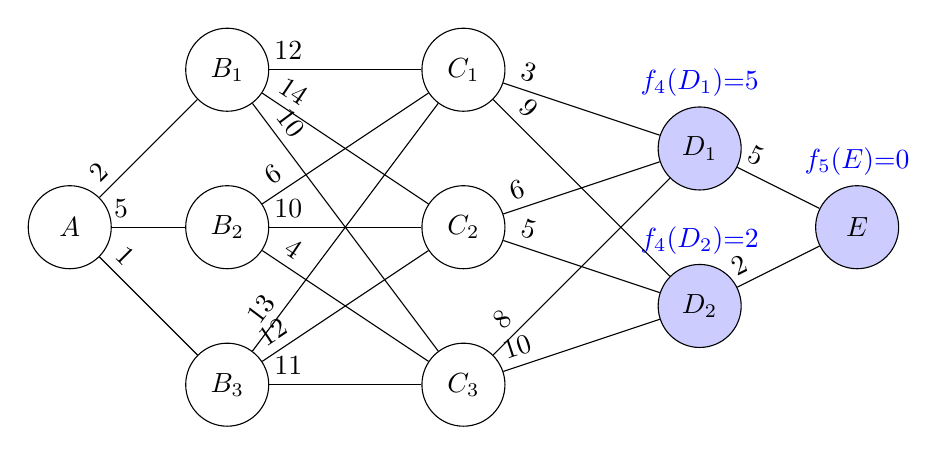
\begin{tikzpicture}[every label/.style={blue}]
        \node[CC1] (1) at(0,0){$A$};
        \node[CC1] (2) at(2,2){$B_1$};
        \node[CC1] (3) at(2,0){$B_2$};
        \node[CC1] (4) at(2,-2){$B_3$};
        \node[CC1] (5) at(5,2){$C_1$};
        \node[CC1] (6) at(5,0){$C_2$};
        \node[CC1] (7) at(5,-2){$C_3$};
        \node[CC2] (8)[label=above:$f_4(D_1){=}5$] at(8,1){$D_1$};
        \node[CC2] (9)[label=above:$f_4(D_2){=}2$] at(8,-1){$D_2$};
        \node[CC2] (10)[label=above:$f_5(E){=}0$] at(10,0){$E$};
        \draw (1) --(2) node[SU]{2};
        \draw (1) --(3) node[SU]{5};
        \draw (1) --(4) node[SU]{1};
        \draw (2) --(5) node[SU]{12};
        \draw (2) --(6) node[SU]{14};
        \draw (2) --(7) node[SU]{10};
        \draw (3) --(5) node[SU]{6};
        \draw (3) --(6) node[SU]{10};
        \draw (3) --(7) node[SU]{4};
        \draw (4) --(5) node[SU]{13};
        \draw (4) --(6) node[SU]{12};
        \draw (4) --(7) node[SU]{11};
        \draw (5) --(8) node[SU]{3};
        \draw (5) --(9) node[SU]{9};
        \draw (6) --(8) node[SU]{6};
        \draw (6) --(9) node[SU]{5};
        \draw (7) --(8) node[SU]{8};
        \draw (7) --(9) node[SU]{10};
        \draw (8) --(10) node[SU]{5};
        \draw (9) --(10) node[SU]{2};
    \end{tikzpicture}
\end{frame}
\begin{frame}{4-2-4}
    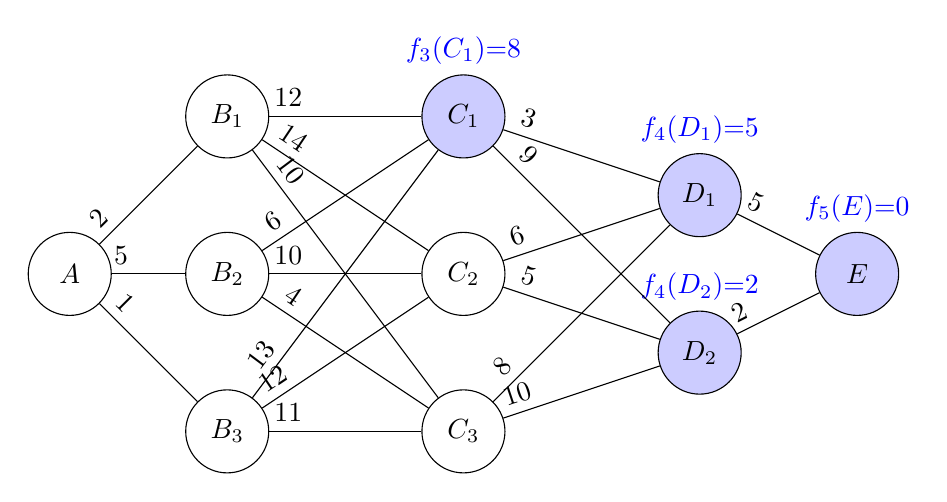
\begin{tikzpicture}[every label/.style={blue}]
        \node[CC1] (1) at(0,0){$A$};
        \node[CC1] (2) at(2,2){$B_1$};
        \node[CC1] (3) at(2,0){$B_2$};
        \node[CC1] (4) at(2,-2){$B_3$};
        \node[CC2] (5)[label=above:$f_3(C_1){=}8$] at(5,2){$C_1$};
        \node[CC1] (6) at(5,0){$C_2$};
        \node[CC1] (7) at(5,-2){$C_3$};
        \node[CC2] (8)[label=above:$f_4(D_1){=}5$] at(8,1){$D_1$};
        \node[CC2] (9)[label=above:$f_4(D_2){=}2$] at(8,-1){$D_2$};
        \node[CC2] (10)[label=above:$f_5(E){=}0$] at(10,0){$E$};
        \draw (1) --(2) node[SU]{2};
        \draw (1) --(3) node[SU]{5};
        \draw (1) --(4) node[SU]{1};
        \draw (2) --(5) node[SU]{12};
        \draw (2) --(6) node[SU]{14};
        \draw (2) --(7) node[SU]{10};
        \draw (3) --(5) node[SU]{6};
        \draw (3) --(6) node[SU]{10};
        \draw (3) --(7) node[SU]{4};
        \draw (4) --(5) node[SU]{13};
        \draw (4) --(6) node[SU]{12};
        \draw (4) --(7) node[SU]{11};
        \draw (5) --(8) node[SU]{3};
        \draw (5) --(9) node[SU]{9};
        \draw (6) --(8) node[SU]{6};
        \draw (6) --(9) node[SU]{5};
        \draw (7) --(8) node[SU]{8};
        \draw (7) --(9) node[SU]{10};
        \draw (8) --(10) node[SU]{5};
        \draw (9) --(10) node[SU]{2};
    \end{tikzpicture}
\end{frame}
\begin{frame}{4-2-5}
    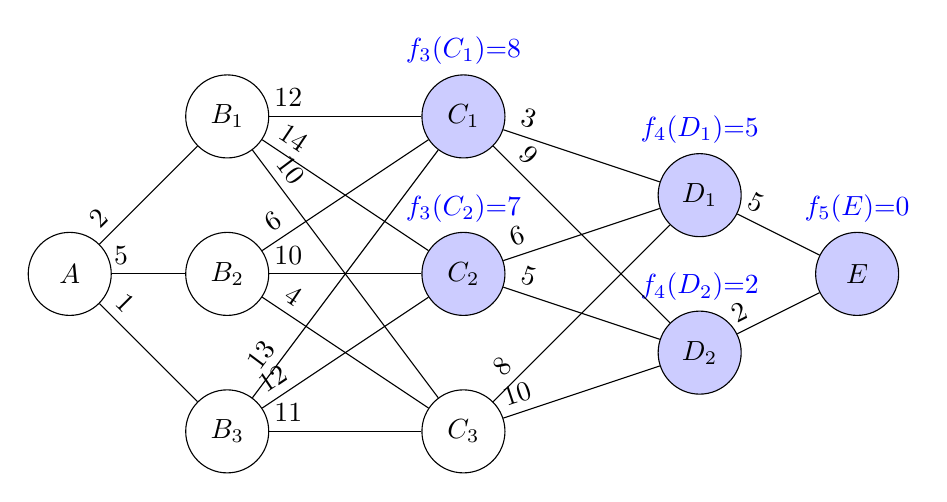
\begin{tikzpicture}[every label/.style={blue}]
        \node[CC1] (1) at(0,0){$A$};
        \node[CC1] (2) at(2,2){$B_1$};
        \node[CC1] (3) at(2,0){$B_2$};
        \node[CC1] (4) at(2,-2){$B_3$};
        \node[CC2] (5)[label=above:$f_3(C_1){=}8$] at(5,2){$C_1$};
        \node[CC2] (6)[label=above:$f_3(C_2){=}7$] at(5,0){$C_2$};
        \node[CC1] (7) at(5,-2){$C_3$};
        \node[CC2] (8)[label=above:$f_4(D_1){=}5$] at(8,1){$D_1$};
        \node[CC2] (9)[label=above:$f_4(D_2){=}2$] at(8,-1){$D_2$};
        \node[CC2] (10)[label=above:$f_5(E){=}0$] at(10,0){$E$};
        \draw (1) --(2) node[SU]{2};
        \draw (1) --(3) node[SU]{5};
        \draw (1) --(4) node[SU]{1};
        \draw (2) --(5) node[SU]{12};
        \draw (2) --(6) node[SU]{14};
        \draw (2) --(7) node[SU]{10};
        \draw (3) --(5) node[SU]{6};
        \draw (3) --(6) node[SU]{10};
        \draw (3) --(7) node[SU]{4};
        \draw (4) --(5) node[SU]{13};
        \draw (4) --(6) node[SU]{12};
        \draw (4) --(7) node[SU]{11};
        \draw (5) --(8) node[SU]{3};
        \draw (5) --(9) node[SU]{9};
        \draw (6) --(8) node[SU]{6};
        \draw (6) --(9) node[SU]{5};
        \draw (7) --(8) node[SU]{8};
        \draw (7) --(9) node[SU]{10};
        \draw (8) --(10) node[SU]{5};
        \draw (9) --(10) node[SU]{2};
    \end{tikzpicture}
\end{frame}
\begin{frame}{4-2-6}
    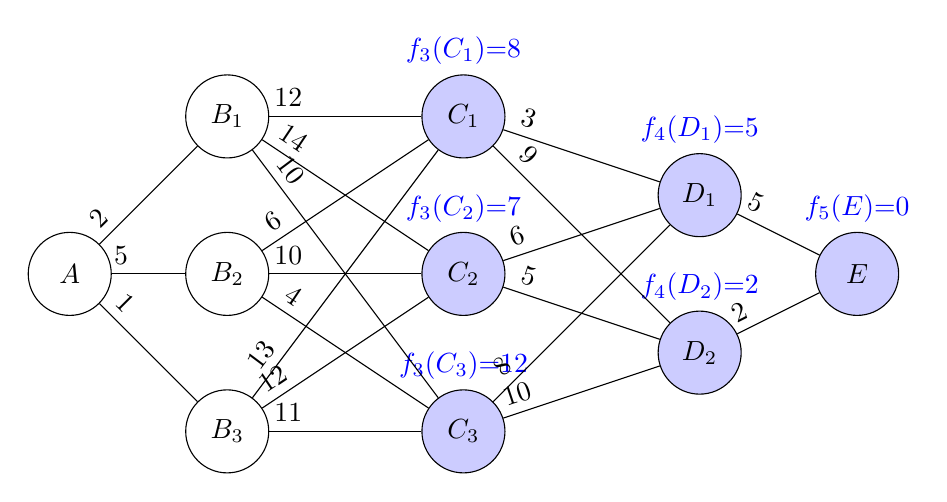
\begin{tikzpicture}[every label/.style={blue}]
        \node[CC1] (1) at(0,0){$A$};
        \node[CC1] (2) at(2,2){$B_1$};
        \node[CC1] (3) at(2,0){$B_2$};
        \node[CC1] (4) at(2,-2){$B_3$};
        \node[CC2] (5)[label=above:$f_3(C_1){=}8$] at(5,2){$C_1$};
        \node[CC2] (6)[label=above:$f_3(C_2){=}7$] at(5,0){$C_2$};
        \node[CC2] (7)[label=above:$f_3(C_3){=}12$] at(5,-2){$C_3$};
        \node[CC2] (8)[label=above:$f_4(D_1){=}5$] at(8,1){$D_1$};
        \node[CC2] (9)[label=above:$f_4(D_2){=}2$] at(8,-1){$D_2$};
        \node[CC2] (10)[label=above:$f_5(E){=}0$] at(10,0){$E$};
        \draw (1) --(2) node[SU]{2};
        \draw (1) --(3) node[SU]{5};
        \draw (1) --(4) node[SU]{1};
        \draw (2) --(5) node[SU]{12};
        \draw (2) --(6) node[SU]{14};
        \draw (2) --(7) node[SU]{10};
        \draw (3) --(5) node[SU]{6};
        \draw (3) --(6) node[SU]{10};
        \draw (3) --(7) node[SU]{4};
        \draw (4) --(5) node[SU]{13};
        \draw (4) --(6) node[SU]{12};
        \draw (4) --(7) node[SU]{11};
        \draw (5) --(8) node[SU]{3};
        \draw (5) --(9) node[SU]{9};
        \draw (6) --(8) node[SU]{6};
        \draw (6) --(9) node[SU]{5};
        \draw (7) --(8) node[SU]{8};
        \draw (7) --(9) node[SU]{10};
        \draw (8) --(10) node[SU]{5};
        \draw (9) --(10) node[SU]{2};
    \end{tikzpicture}
\end{frame}
\begin{frame}{4-2-7}
    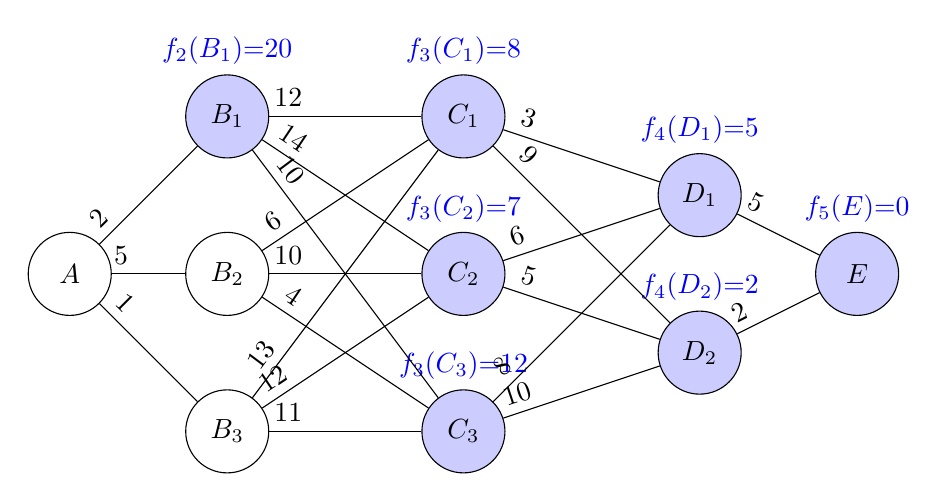
\begin{tikzpicture}[every label/.style={blue}]
        \node[CC1] (1) at(0,0){$A$};
        \node[CC2] (2)[label=above:$f_2(B_1){=}20$] at(2,2){$B_1$};
        \node[CC1] (3) at(2,0){$B_2$};
        \node[CC1] (4) at(2,-2){$B_3$};
        \node[CC2] (5)[label=above:$f_3(C_1){=}8$] at(5,2){$C_1$};
        \node[CC2] (6)[label=above:$f_3(C_2){=}7$] at(5,0){$C_2$};
        \node[CC2] (7)[label=above:$f_3(C_3){=}12$] at(5,-2){$C_3$};
        \node[CC2] (8)[label=above:$f_4(D_1){=}5$] at(8,1){$D_1$};
        \node[CC2] (9)[label=above:$f_4(D_2){=}2$] at(8,-1){$D_2$};
        \node[CC2] (10)[label=above:$f_5(E){=}0$] at(10,0){$E$};
        \draw (1) --(2) node[SU]{2};
        \draw (1) --(3) node[SU]{5};
        \draw (1) --(4) node[SU]{1};
        \draw (2) --(5) node[SU]{12};
        \draw (2) --(6) node[SU]{14};
        \draw (2) --(7) node[SU]{10};
        \draw (3) --(5) node[SU]{6};
        \draw (3) --(6) node[SU]{10};
        \draw (3) --(7) node[SU]{4};
        \draw (4) --(5) node[SU]{13};
        \draw (4) --(6) node[SU]{12};
        \draw (4) --(7) node[SU]{11};
        \draw (5) --(8) node[SU]{3};
        \draw (5) --(9) node[SU]{9};
        \draw (6) --(8) node[SU]{6};
        \draw (6) --(9) node[SU]{5};
        \draw (7) --(8) node[SU]{8};
        \draw (7) --(9) node[SU]{10};
        \draw (8) --(10) node[SU]{5};
        \draw (9) --(10) node[SU]{2};
    \end{tikzpicture}
\end{frame}
\begin{frame}{4-2-8}
    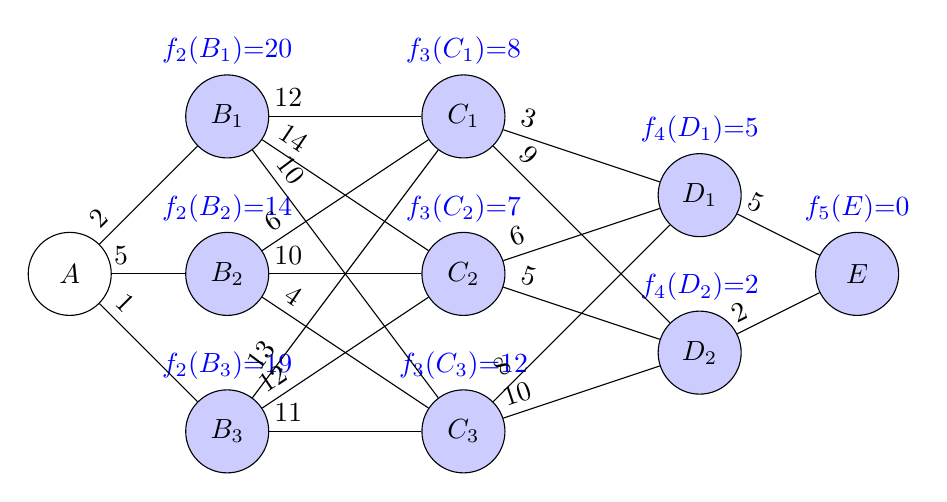
\begin{tikzpicture}[every label/.style={blue}]
        \node[CC1] (1) at(0,0){$A$};
        \node[CC2] (2)[label=above:$f_2(B_1){=}20$] at(2,2){$B_1$};
        \node[CC2] (3)[label=above:$f_2(B_2){=}14$] at(2,0){$B_2$};
        \node[CC2] (4)[label=above:$f_2(B_3){=}19$] at(2,-2){$B_3$};
        \node[CC2] (5)[label=above:$f_3(C_1){=}8$] at(5,2){$C_1$};
        \node[CC2] (6)[label=above:$f_3(C_2){=}7$] at(5,0){$C_2$};
        \node[CC2] (7)[label=above:$f_3(C_3){=}12$] at(5,-2){$C_3$};
        \node[CC2] (8)[label=above:$f_4(D_1){=}5$] at(8,1){$D_1$};
        \node[CC2] (9)[label=above:$f_4(D_2){=}2$] at(8,-1){$D_2$};
        \node[CC2] (10)[label=above:$f_5(E){=}0$] at(10,0){$E$};
        \draw (1) --(2) node[SU]{2};
        \draw (1) --(3) node[SU]{5};
        \draw (1) --(4) node[SU]{1};
        \draw (2) --(5) node[SU]{12};
        \draw (2) --(6) node[SU]{14};
        \draw (2) --(7) node[SU]{10};
        \draw (3) --(5) node[SU]{6};
        \draw (3) --(6) node[SU]{10};
        \draw (3) --(7) node[SU]{4};
        \draw (4) --(5) node[SU]{13};
        \draw (4) --(6) node[SU]{12};
        \draw (4) --(7) node[SU]{11};
        \draw (5) --(8) node[SU]{3};
        \draw (5) --(9) node[SU]{9};
        \draw (6) --(8) node[SU]{6};
        \draw (6) --(9) node[SU]{5};
        \draw (7) --(8) node[SU]{8};
        \draw (7) --(9) node[SU]{10};
        \draw (8) --(10) node[SU]{5};
        \draw (9) --(10) node[SU]{2};
    \end{tikzpicture}
\end{frame}
\begin{frame}{4-2-9}
    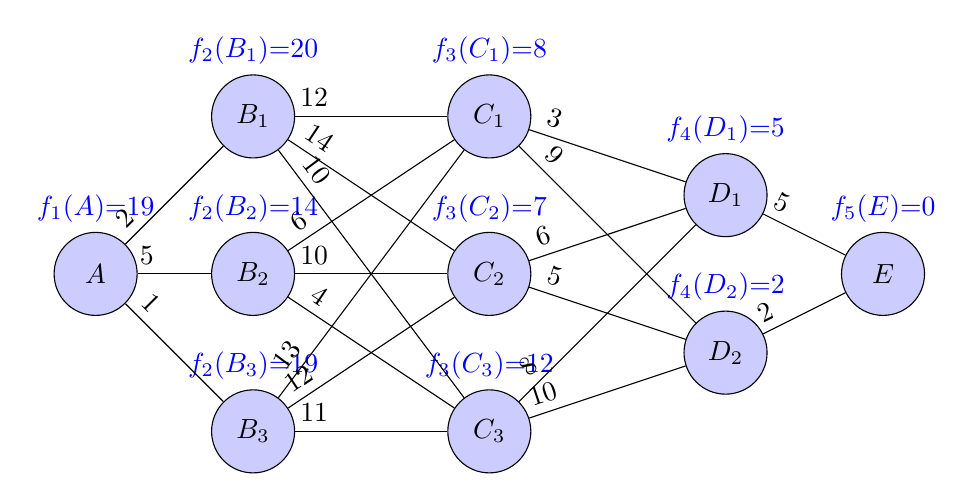
\begin{tikzpicture}[every label/.style={blue}]
        \node[CC2] (1)[label=above:$f_1(A){=}19$] at(0,0){$A$};
        \node[CC2] (2)[label=above:$f_2(B_1){=}20$] at(2,2){$B_1$};
        \node[CC2] (3)[label=above:$f_2(B_2){=}14$] at(2,0){$B_2$};
        \node[CC2] (4)[label=above:$f_2(B_3){=}19$] at(2,-2){$B_3$};
        \node[CC2] (5)[label=above:$f_3(C_1){=}8$] at(5,2){$C_1$};
        \node[CC2] (6)[label=above:$f_3(C_2){=}7$] at(5,0){$C_2$};
        \node[CC2] (7)[label=above:$f_3(C_3){=}12$] at(5,-2){$C_3$};
        \node[CC2] (8)[label=above:$f_4(D_1){=}5$] at(8,1){$D_1$};
        \node[CC2] (9)[label=above:$f_4(D_2){=}2$] at(8,-1){$D_2$};
        \node[CC2] (10)[label=above:$f_5(E){=}0$] at(10,0){$E$};
        \draw (1) --(2) node[SU]{2};
        \draw (1) --(3) node[SU]{5};
        \draw (1) --(4) node[SU]{1};
        \draw (2) --(5) node[SU]{12};
        \draw (2) --(6) node[SU]{14};
        \draw (2) --(7) node[SU]{10};
        \draw (3) --(5) node[SU]{6};
        \draw (3) --(6) node[SU]{10};
        \draw (3) --(7) node[SU]{4};
        \draw (4) --(5) node[SU]{13};
        \draw (4) --(6) node[SU]{12};
        \draw (4) --(7) node[SU]{11};
        \draw (5) --(8) node[SU]{3};
        \draw (5) --(9) node[SU]{9};
        \draw (6) --(8) node[SU]{6};
        \draw (6) --(9) node[SU]{5};
        \draw (7) --(8) node[SU]{8};
        \draw (7) --(9) node[SU]{10};
        \draw (8) --(10) node[SU]{5};
        \draw (9) --(10) node[SU]{2};
    \end{tikzpicture}
\end{frame}
\begin{frame}{4-2-10}
    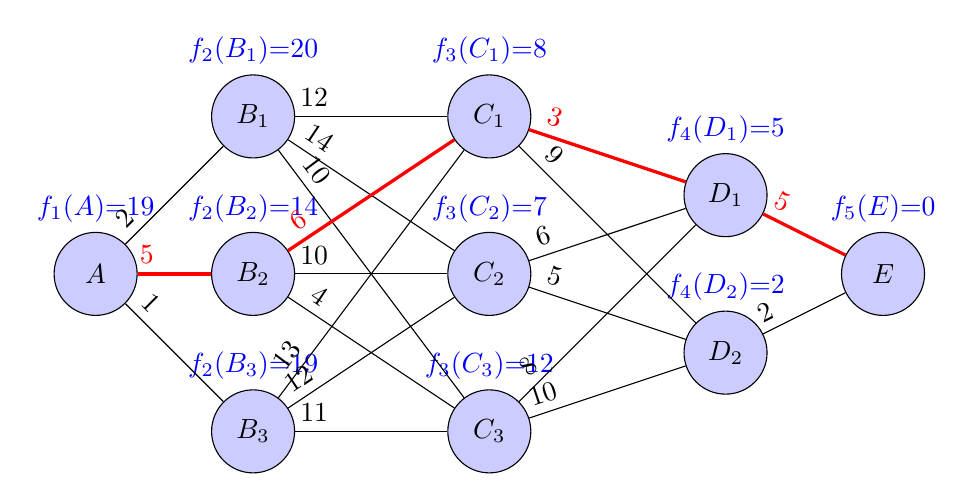
\begin{tikzpicture}[every label/.style={blue}]
        \node[CC2] (1)[label=above:$f_1(A){=}19$] at(0,0){$A$};
        \node[CC2] (2)[label=above:$f_2(B_1){=}20$] at(2,2){$B_1$};
        \node[CC2] (3)[label=above:$f_2(B_2){=}14$] at(2,0){$B_2$};
        \node[CC2] (4)[label=above:$f_2(B_3){=}19$] at(2,-2){$B_3$};
        \node[CC2] (5)[label=above:$f_3(C_1){=}8$] at(5,2){$C_1$};
        \node[CC2] (6)[label=above:$f_3(C_2){=}7$] at(5,0){$C_2$};
        \node[CC2] (7)[label=above:$f_3(C_3){=}12$] at(5,-2){$C_3$};
        \node[CC2] (8)[label=above:$f_4(D_1){=}5$] at(8,1){$D_1$};
        \node[CC2] (9)[label=above:$f_4(D_2){=}2$] at(8,-1){$D_2$};
        \node[CC2] (10)[label=above:$f_5(E){=}0$] at(10,0){$E$};
        \draw (1) --(2) node[SU]{2};
        \draw[red,very thick] (1) --(3) node[SU]{5};
        \draw (1) --(4) node[SU]{1};
        \draw (2) --(5) node[SU]{12};
        \draw (2) --(6) node[SU]{14};
        \draw (2) --(7) node[SU]{10};
        \draw (3) --(5)[red,very thick] node[SU]{6};
        \draw (3) --(6) node[SU]{10};
        \draw (3) --(7) node[SU]{4};
        \draw (4) --(5) node[SU]{13};
        \draw (4) --(6) node[SU]{12};
        \draw (4) --(7) node[SU]{11};
        \draw[red,very thick] (5) --(8) node[SU]{3};
        \draw (5) --(9) node[SU]{9};
        \draw (6) --(8) node[SU]{6};
        \draw (6) --(9) node[SU]{5};
        \draw (7) --(8) node[SU]{8};
        \draw (7) --(9) node[SU]{10};
        \draw[red,very thick] (8) --(10) node[SU]{5};
        \draw (9) --(10) node[SU]{2};
    \end{tikzpicture}
\end{frame}
\begin{frame}{4-3}
    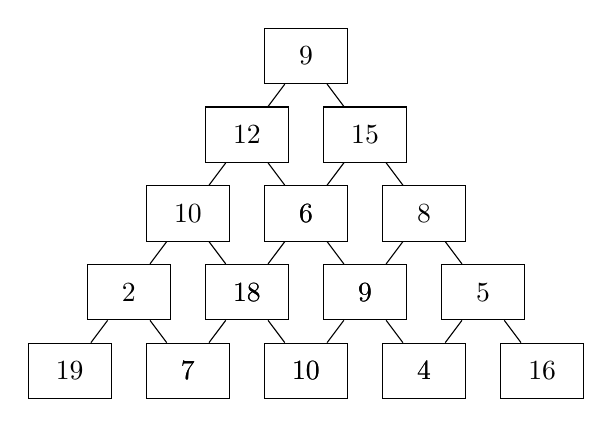
\begin{tikzpicture}
        [every node/.style={rectangle,minimum width = 30pt, minimum height =20pt,draw},
        level distance= 1cm]
        \node{9}
            child{node{12}
                child{node{10}
                    child{node{2} child{node{19}} child{node{7}}}
                    child{node{18} child{node{7}} child{node{10}}}}
                    child{node{6}
                    child{node{18}}
                    child{node{9} child{node{10}} child{node{4}}}}    
                    }
                child{node{15}
                    child{node{6}}
                    child{node{8}
                    child{node{9}}
                    child{node{5} child{node{4}} child{node{16}}}}    
                    };
        \end{tikzpicture}
\end{frame}
\begin{frame}{4-4}
    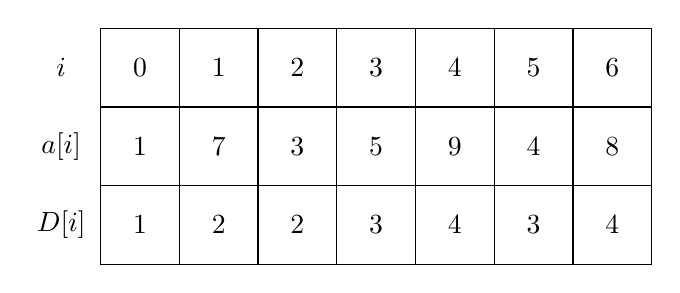
\begin{tikzpicture}
        \draw (0,0) node[RA2]{1};
        \draw (1,0) node[RA2]{2};
        \draw (2,0) node[RA2]{2};
        \draw (3,0) node[RA2]{3};
        \draw (4,0) node[RA2]{4};
        \draw (5,0) node[RA2]{3};
        \draw (6,0) node[RA2]{4};
        \node at (-1,0) {$D[i]$};
        \draw (0,1) node[RA2]{1};
        \draw (1,1) node[RA2]{7};
        \draw (2,1) node[RA2]{3};
        \draw (3,1) node[RA2]{5};
        \draw (4,1) node[RA2]{9};
        \draw (5,1) node[RA2]{4};
        \draw (6,1) node[RA2]{8};
        \node at (-1,1) {$a[i]$};
        \foreach \x in {0,...,6}{
            \draw (\x,2) node[RA2]{\x};}
        \node at (-1,2) {$i$};
    \end{tikzpicture}
\end{frame}
\begin{frame}{4-5}
    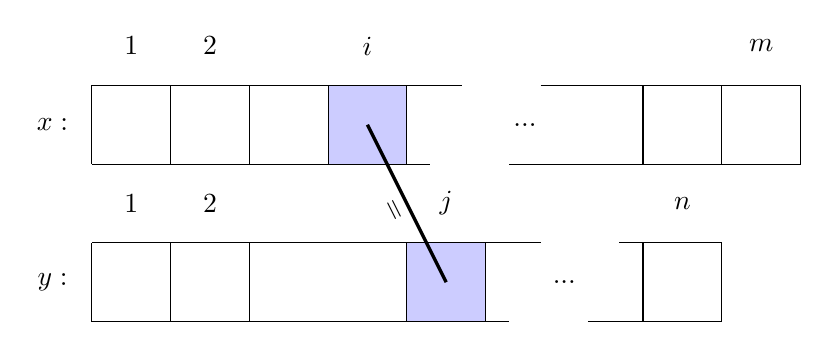
\begin{tikzpicture}
        \draw (0,0) --(5.3,0);
        \draw (0,1) --(5.7,1);
        \draw (0,2) --(4.3,2);
        \draw (0,3) --(4.7,3);
        \draw (6.3,0) --(8,0);
        \draw (6.7,1) --(8,1);
        \draw (5.3,2) --(9,2);
        \draw (5.7,3) --(9,3);
        \foreach \x in {0,1,2,7,8}
            \foreach \y in {0,2}{
                \draw (0+\x,0+\y) --(0+\x,1+\y);}
        \draw (9,2) --(9,3);
        \node at (-.5,0.5) {$y:$};
        \node at (-.5,2.5) {$x:$};
        \foreach \x in {1,2}
            \foreach \y in {0,2}{
                \node at (-.5+\x,1.5+\y) {$\x$};}   
        \node at (3.5,3.5) {$i$};
        \node at (4.5,1.5) {$j$};
        \node at (8.5,3.5) {$m$};
        \node at (7.5,1.5) {$n$};
        \node at (6,0.5) {...}; 
        \node at (5.5,2.5) {...}; 
        \node[RA2,fill=blue!20] at (4.5,0.5){} ; 
        \node[RA2,fill=blue!20] at (3.5,2.5){} ; 
        \draw[very thick] (3.5,2.5) --(4.5,.5) node[midway,below,sloped]{$=$};
    \end{tikzpicture}
\end{frame}
\begin{frame}{5-1}
    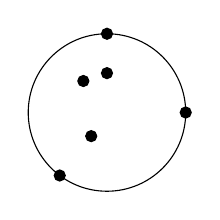
\begin{tikzpicture}
        \filldraw (0,.5) circle[radius=2pt]
        (0,.5) circle[radius=2pt]
        (0,1) circle[radius=2pt]
        (0,.5) circle[radius=2pt]
        (1,0) circle[radius=2pt]
        (-.6,-.8) circle[radius=2pt]
        (-.3,.4) circle[radius=2pt]
        (-.2,-.3) circle[radius=2pt];
        \draw (0,0) circle[radius=1];
    \end{tikzpicture}
\end{frame}
\begin{frame}{5-2}
    \begin{tikzpicture}
        {[ultra thick]{
        \draw (5,6)--(6,6);
        \draw (1,5.5)--(4,5.5);
        \draw (9.9,5)--(10.1,5);
        \draw (6,4.5)--(9,4.5);
        \draw (8,4)--(10,4);}}
        \draw (1,3.5)--(10,3.5);
        \foreach \x in {1,...,10}{
            \draw (\x,3.5)--(\x,3.6);
            \node at (\x,3.2){\x};}
        \draw[ultra thick,blue] (1,2)--(4,2);
        \draw[ultra thick,blue] (5,1.5)--(10,1.5);
        \draw (1,1)--(10,1);
        \foreach \x in {1,...,10}{
            \draw (\x,1)--(\x,1.1);
            \node at (\x,.7){\x};}
    \end{tikzpicture}
\end{frame}
\end{document}
